\section{Hardware evaluation}\label{hardware-evaluation}

\subsection{Qualitative discussion of weather station performance}

\subsubsection{Battery life, solar power and
  outages}\label{sec:hardware-evaluation-power}

The nodes have had more downtime than expected based on the energy budgets in
Sections~\ref{sec:battery-tests} and~\ref{sec:solar-tests}, despite doubling the
battery capacity during deployment. The primary cause is site placement, with
both nodes in a north-facing garden bounded by 2.5\,m fencing and a two-storey
house immediately to the south. As a result, they receive no direct sunlight
until 09:00, and Node 1 is shaded again by 15:00 due to the shadow of a nearby
garage. This leaves only \(\approx\)5\,h of direct sunlight, which is far below
the amount assumed in the design of the nodes.

Outages seem to only affect the sensor nodes; the repeater has had zero downtime
since installation. This is consistent with its much lower energy budget from a
lack of any peripheral sensors, which reduces average energy draw.

The limitations of the current location, plausibly explain the observed outages.
Because these shading conditions are unlikely in an open field, these outages
are not of primary concern for the intended deployment. However, it highlights
the system's sensitivity to late sunrise and early sunsets from terrain. This
would potentially be an issue if the actual deploy site was shaded by a hill or
some tall trees late in the day, which I had not properly considered in the
design phase.

\subsubsection{Weatherproofing}

The summer of 2025 is set to be one of the hottest and driest on record with
August specifically receiving roughly half its average rainfall
\cite{uor2025summer}. Consequently, from the 15th of August to the 26th of
August the weather stations saw only short spells of rain, making an analysis of
their weather proofing hard to review up to this point.

Fortunately, from the 27th August onwards the nodes were exposed to fairly heavy
sustained rainfall. Throughout this period there has been no evidence of water
ingress.

Beyond ingress testing, the nodes experienced elevated ambient temperatures
(exceeding \SI{32}{\degreeCelsius}) and showed no signs of overheating. These
results are encouraging, although longer-term deployment that includes colder
weather and sustained heavy rain is needed to comment conclusively on their
overall robustness.

\subsubsection{Range}\label{sec:range-eval}

As reported in section ~\ref{sec:range-tests} the Challenger microcontrollers
and antennas used in this configuration are able to reach at least 1200m of
range in a real world situation. The conditions in that test were not ideal for
LoRa as both the receiver and transmitter were positioned low to the ground at
around 1-1.5m. In addition line of sight was broken at around 1000m which
severely diminishes the performance of any radio communication system. There
were also buildings between 1200m and 1400m that blocked LoRa signals entirely.

In the intended deployment of my full weather network, the use of an additional
repeater would significantly improve range. In a flat terrain setting the use of
a repeater would double the range. If terrain is hilly a repeater can increase
range by even larger multiples. The below graphic demonstrates the problem of
hills when it comes to LoRa. As a LoRa signal propagates from the transmitter
and collides with a hill the majority of the signals energy is reflected off the
hill meaning it cannot reach the gateway.

\begin{figure}[H]
  \centering
  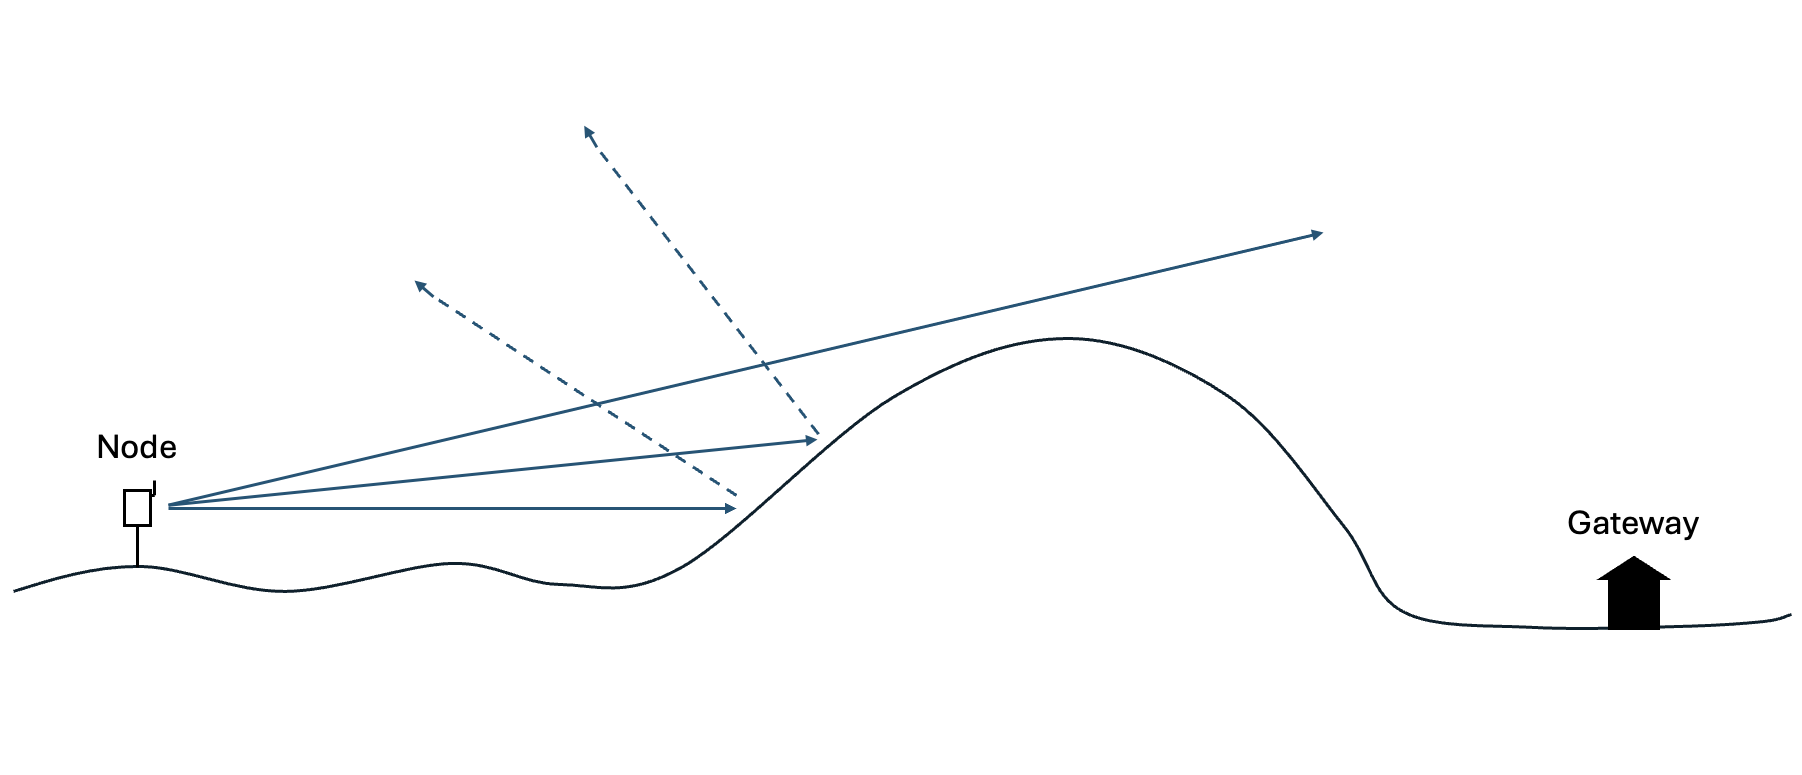
\includegraphics[width=0.9\textwidth]{contents/part-4/fig4/no-repeater.png}
  \caption{Illustration of LoRa radio propagation between node and receiver with blocking terrain}
  \label{fig:no-repeater}
\end{figure}

If a repeater is placed on the top of the hill not only would it mean the LoRa
signal would reach the gateway but the repeaters increased elevation would give
a significant boost to its range as the total area with a line of sight to the
repeater would be vastly increased.

The range that this repeater allows is what sets the design of my network apart
from commercial options and is discussed in more detail in the next section..

\begin{figure}[H]
  \centering
  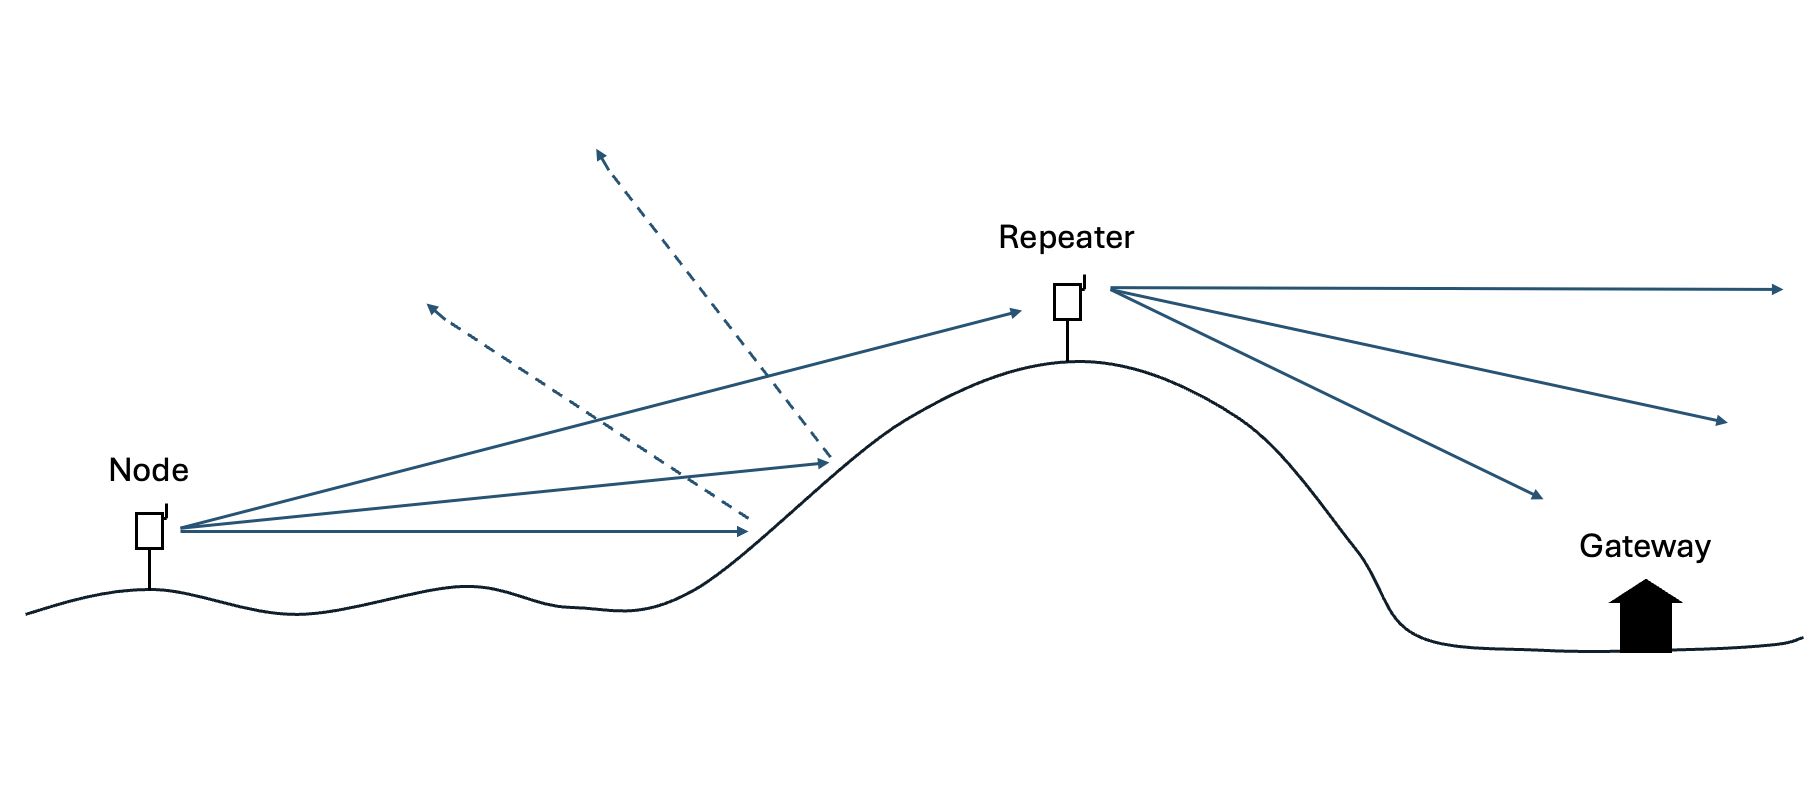
\includegraphics[width=0.9\textwidth]{contents/part-4/fig4/repeater.png}
  \caption{Illustration of LoRa radio propagation with a repeater included}
  \label{fig:repeater}
\end{figure}

\subsubsection{Reset behaviour}\label{sec:reset-behaviour}

As covered briefly in Chapter~\ref{sec:deployment}, the reset behaviour of the
Challenger is inconsistent after a brownout or complete power outage.
Essentially if the sensor nodes run out of power, there is no certainty that the
node will restart the code.py program when power returns. This is in spite of
the fact that I modified the safemode.py behaviour of CircuitPython with the
recommended code for remote solar power applications. As this ultimately appears
to be a firmware issue there is not an obvious or easy solution for this.

With enough time I would probably rewrite all of the Challenger software in
MicroPython and see if that firmware behaves in a more reliable and
deterministic way on power outage. Unfortunately the issue was picked up fairly
late in development and it was unrealistic to perform a refactor of this scale
with the time left.

\subsection{Quantitative comparison with commercial alternatives}

I will now compare the performance of my LoRa weather station to prebuilt
options available to purchase. A breakdown of costs for Agriscanner is included
in Appendix~\ref{app:cost-nodes}.

\begin{table}[H]
  \centering
  \small
  \renewcommand{\arraystretch}{1.2}
  \begin{tabularx}{\textwidth}{l >{\raggedright\arraybackslash}X
      >{\raggedright\arraybackslash}X >{\raggedright\arraybackslash}X
      >{\raggedright\arraybackslash}X >{\raggedright\arraybackslash}X}
    \hline
                                                    & \textbf{Agriscanner
    Network}                                        & \textbf{SenseCAP
    S2120\cite{pihut:sensecap-s2120-2025}}          & \textbf{Decentlab Eleven
    Parameter\cite{alliot:decentlab-eleven-2025}}   & \textbf{HOBO weather
    station kit\cite{weathershop:hobo-rx3000-2025}} & \textbf{SparkFun Arduino
    weather kit\cite{pihut:sparkfun-2025}}
    \\

    \hline
    Number of sensors                               & 4
    & 8                     & 11\textsuperscript{*}                           &
    6                         & 7                                \\
    Sensor accuracy                                 & Hobbyist
                                                    & Hobbyist & Professional
                                                    & Professional          &
                                                    Hobbyist \\
    Communication type                              & LoRa
                                                    & LoRa & LoRa
                                                    & Mobile network        &
                                                    WiFi \\
    Update frequency                                & 1 minute
                                                    & 1 hour & 10 minutes
                                                    & 1 hour & 1 minute
                                                    \\
    Readings per hour                               & 60
    & 1                     & 6                                               &
    10                        & 60                               \\
    Power source included                           & Yes
    & Yes                   & Yes                                             &
    Yes                       & No                               \\
    Power source                                    & Solar
                                                    & Solar & Solar
                                                    & Solar                 & --
                                                    \\
    Batteries recharge?                             & Yes
    & No                    & No                                              &
    Yes                       & --                               \\
    Reported battery life                           & replace $\sim$ 3 years
    & 154 days                                        & Several months
    & replace 3--5 years                                      & --
    \\
    Reported range                                  & --
    & 2--10\,km             & 2--10\,km                                       &
    Anywhere with 4G & --
    \\
    Estimated range                                 & 2.4--20\,km
                                                    & 1.2--10\,km & 1.2--10\,km
                                                    & -- & 10--50\,m
                                                    \\
    IP rating                                       & $\sim$ IP65
                                                    & IPX6 & IP66
                                                    & IP66                  &
                                                    None     \\
    Ongoing payment?                                & --
    & --                    & --                                              &
    Yes -- mobile plan        & -- \\
    Ongoing costs p.a                               & \pounds{}0
                                                    & \pounds{}0 & \pounds{}0
                                                    & \pounds{}132 & \pounds{}0
                                                    \\
    Cost per sensor node                            & \pounds{}177
    & \pounds{}287                                    & \pounds{}3{,}272
    & \pounds{}4{,}138                                & \pounds{}130
    \\
    Cost per repeater                               & \pounds{}93
                                                    & \pounds{}0 & \pounds{}0
                                                    & \pounds{}0 & \pounds{}0
                                                    \\
    Cost per gateway\textsuperscript{**}            & \pounds{}66
                                                    & \pounds{}122 &
                                                    \pounds{}122 & \pounds{}0
                                                    & \pounds{}0
                                                    \\
    Battery cost p.a.\textsuperscript{***}          & \pounds{}7
                                                    & \pounds{}10 & \pounds{}30
                                                    & \pounds{}20 & \pounds{}0
                                                    \\
    \textbf{Total cost\textsuperscript{****}}       & \textbf{\pounds{}520}
    & \textbf{\pounds{}706}                           &
    \textbf{\pounds{}6{,}696} & \textbf{\pounds{}8{,}418} &
    \textbf{\pounds{}260} \\
    \hline
  \end{tabularx}

  \vspace{0.25em}
  \textit{\footnotesize * Sensors missing from Agriscanner: Solar radiation,
    rainfall, barometric pressure, vapor pressure, dew point, wind direction,
    tilt sensor, lightning strike count / distance} \\
  \textit{\footnotesize ** For SenseCAP and Decentlab models the lowest cost
    gateway available is sensecap m2 at £122} \\
  \textit{\footnotesize *** Battery cost assumptions are detailed in
    Appendix~\ref{app:battery-assumptions}.} \\
  \textit{\footnotesize **** Includes sensors, repeater, gateway, and estimated first-year battery + ongoing costs.}
  \caption{Comparison of weather-station options.}
  \label{tab:commercial-comparison}
\end{table}

\subsubsection{Benefits of my weather station}

\begin{itemize}
  \item \textbf{Cost:} At £520 the Agriscanner weather stations are the lowest
        cost option among waterproof, long-range systems. While the SparkFun kit
        is cheaper, it is not suitable for outdoor deployment due to its exposed
        electronics and, since it relies on WiFi, its range would be
        insufficient in an agricultural setting. It will therefore not be
        discussed further. The two professional systems (DecentLab and HOBO) are
        over ten times the price of my system and are therefore not comparable.

        The only system with similar characteristics under £1,000 that I could
        find is the SenseCAP device. However, with a cost per node roughly 50\%
        higher, my nodes still provide better value. If additional nodes were
        deployed, this price difference would become even more significant.

  \item \textbf{Frequency of readings:} My sensor nodes collect and transmit
        readings every minute, providing the Agriscanner webapp with effectively
        live data. By contrast, most alternative options only provide hourly
        readings, leaving actual conditions between measurements unknown.

  \item \textbf{Battery recharging:} My nodes use rechargeable 18650 batteries,
        which I conservatively estimate will last around three years (they use
        the same battery chemistry as mobile phones) before requiring
        replacement. Of the alternatives, only the HOBO system features a
        rechargeable battery. Both SenseCAP and DecentLab rely on disposable
        alkaline batteries, requiring regular replacement and therefore more
        frequent maintenance.

  \item \textbf{Range:} As explained in Section~\ref{sec:range-eval}, my weather
        station network benefits from the inclusion of a repeater. This enables
        significantly greater range than the other models could provide,
        particularly in hilly terrain.

        I also doubt whether either the SenseCAP or DecentLab systems could
        achieve a substantial range improvement under the same test conditions.
        In the UK, LoRa transmission power is subject to a strict regulatory cap
        (see Section~\ref{sec:lora-limit}). Since my system already operates at
        this maximum power, commercial products cannot exceed it. Even with a
        superior antenna, transmit power would need to be reduced
        proportionally, as antenna gain also counts towards the effective
        radiated power. It is therefore highly unlikely that these alternatives
        would achieve a range advantage sufficient to offset the benefits of a
        repeater in my system.
\end{itemize}

\subsubsection{Drawbacks of my weather station}

\begin{itemize}
  \item \textbf{Number of sensors:} One of the clearest drawbacks of the
        Agriscanner system is the lower sensor count: only four sensors compared
        with seven to eleven on competing systems. However, the Challenger
        microcontrollers in my sensor nodes still have spare GPIO ports, so
        adding additional sensors would be straightforward. The cost of many
        sensors is also not prohibitive (for example, a UV index sensor is only
        \pounds{}6).
  \item \textbf{Sensor accuracy:} Professional systems use higher-grade sensors
        with tighter accuracy specs. For example, the DecentLab unit specifies
        air temperature accuracy of $\pm0.6\,\si{\celsius}$, whereas the DHT11
        used in mine is only rated to about $\pm2.0\,\si{\celsius}$.
  \item \textbf{Reset behaviour:} As noted in Section~\ref{sec:reset-behaviour},
        the node firmware can behave unreliably after a full battery drain.
        While I cannot purchase the other devices in this list to confirm this
        directly, it is unlikely that the other units would exhibit the same
        behaviour, especially because their firmware will have been built
        specifically for remote solar powered applications.
  \item \textbf{Remote Health Diagnostics:} The Agriscanner provides no way to
        remotely monitor battery health and charging status. Such capabilities
        would help diagnose issues caused by poor choice of location for
        effective charging. A location that might have been acceptable at the
        time of installation might become non-viable as the sun becomes lower in
        the sky in the autumn and winter, or as vegetation grows and occludes
        the solar panels.
  \item \textbf{Other factors:} The other devices bring other non-tangible
        benefits besides their technical specification. For example, warranties,
        formal testing, vendor support etc. Professional systems commonly offer
        long-term maintenance and firmware updates beyond the initial purchase,
        which my prototype solution obviously does not offer.
\end{itemize}

\subsection{Conclusion on hardware performance}

While the weather station network has shown promising results as a low cost and
long range solution, the unreliable reset behaviour holds it back from being
100\% deployment ready. So far the weatherproofing of the external devices has
been encouraging, though testing has been limited due to unusually dry weather
and a longer deployment in wetter and colder conditions is needed. The outages
seen during the current deployment appear to be an issue specific to the private
garden they are in and would be much less likely in an open field environment;
however, this does emphasise the need for more extensive site surveys prior to
installation. Overall, if the reset behaviour can be addressed and a small
number of additional sensors are added, the complete system would be well suited
for long term unattended deployment on a farm.